% Template for Cogsci submission with R Markdown

% Stuff changed from original Markdown PLOS Template
\documentclass[10pt, letterpaper]{article}

\usepackage{cogsci}
\usepackage{pslatex}
\usepackage{float}
\usepackage{caption}

% amsmath package, useful for mathematical formulas
\usepackage{amsmath}

% amssymb package, useful for mathematical symbols
\usepackage{amssymb}

% hyperref package, useful for hyperlinks
\usepackage{hyperref}

% graphicx package, useful for including eps and pdf graphics
% include graphics with the command \includegraphics
\usepackage{graphicx}

% Sweave(-like)
\usepackage{fancyvrb}
\DefineVerbatimEnvironment{Sinput}{Verbatim}{fontshape=sl}
\DefineVerbatimEnvironment{Soutput}{Verbatim}{}
\DefineVerbatimEnvironment{Scode}{Verbatim}{fontshape=sl}
\newenvironment{Schunk}{}{}
\DefineVerbatimEnvironment{Code}{Verbatim}{}
\DefineVerbatimEnvironment{CodeInput}{Verbatim}{fontshape=sl}
\DefineVerbatimEnvironment{CodeOutput}{Verbatim}{}
\newenvironment{CodeChunk}{}{}

% cite package, to clean up citations in the main text. Do not remove.
\usepackage{cite}

\usepackage{color}

% Use doublespacing - comment out for single spacing
%\usepackage{setspace}
%\doublespacing


% % Text layout
% \topmargin 0.0cm
% \oddsidemargin 0.5cm
% \evensidemargin 0.5cm
% \textwidth 16cm
% \textheight 21cm

\title{An information-seeking account of eye movements during spoken and signed
language comprehension}


\author{ {\large \bf Kyle MacDonald}$^1$ (kylem4@stanford.edu), {\large \bf Aviva Blonder}$^2$ (aviva.blonder@oberlin.edu), \\ 
  {\large \bf Virginia Marchman}$^1$ (marchman@stanford.edu), {\large \bf Anne Fernald}$^1$ (afernald@stanford.edu), \\ {\large \bf Michael C. Frank}$^1$ (mcfrank@stanford.edu) 
  \\ $^1$ Department of Psychology Stanford University, $^2$ Department of Psychology Oberlin College}

\begin{document}

\maketitle

\begin{abstract}
Language comprehension in grounded contexts involves integrating visual
and linguistic information through decisions about visual fixation. But
when the visual signal also contains information about the language
source -- as in the case of written text or sign language -- how do we
decide where to look? Here, we hypothesize that eye movements during
language comprehension represent an adaptive response. Using two case
studies, we show that, compared to English-learners, young signers
delayed their gaze shifts away from a language source, were more
accurate with these shifts, and produced a smaller proportion of
nonlanguage-driven shifts (E1). Next, we present a well-controlled,
confirmatory experiment, showing that English-speaking adults produced
fewer nonlanguage-driven shifts when processing printed text compared to
spoken language (E2). Together, these data suggest that people adapt to
the value of seeking different information in order to increase the
chance of rapid and accurate language understanding.

\textbf{Keywords:}
eye movements; language processing; information-seeking; American Sign
Language
\end{abstract}

\section{Introduction}\label{introduction}

The study of eye movements during language comprehension has provided
fundamental insights into the interaction between conceptual
representations of the world and the incoming linguistic signal. For
example, research shows that adults and children will rapidly shift
visual attention upon hearing the name of an object in the visual scene,
with a high proportion of shifts occurring prior to the offset of the
word (Allopenna, Magnuson, \& Tanenhaus, 1998; Tanenhaus,
Spivey-Knowlton, Eberhard, \& Sedivy, 1995). Moreover, researchers have
found that conceptual representations activated by fixations to the
visual world can modulate subsequent eye movements during language
processing (Altmann \& Kamide, 2007).

The majority of this work has used eye movements as a measure of the
output of the underlying language comprehension process, often using
linguistic stimuli that come from a disembodied voice. But in real world
contexts, people also gather information about the linguistic signal by
fixating on the language source. Consider a speaker who asks you to
``Pass the salt'' but you are in a noisy room, making it difficult to
understand the request. Here, comprehension can be facilitated by
gathering information via (a) fixations to the nonlinguistic visual
world (i.e., encoding the objects that are present in the scene) or (b)
fixations to the speaker (i.e., reading lips or perhaps the direction of
gaze).

But, this situation creates a tradeoff where the listener must decide
what kind of information to gather and at what time. How do we decide
where to look? We propose that people modulate their eye movements
during language comprehension in response to tradeoffs in the value of
gathering different kinds of information. We test this adaptive tradeoff
account using two case studies that manipulate the value of different
fixation locations for language understanding: a) a comparison of
processing sign vs.~spoken language in children (E1), and b) a
comparison of processing printed text vs.~spoken language in adults
(E2). Our key prediction is that competition for visual attention will
make gaze shifts away from the language source less valuable than
fixating the source of the linguistic signal, leading people to generate
fewer exploratory, nonlanguage-driven eye movements.

\section{Experiment 1}\label{experiment-1}

E1 provides an initial test of our adaptive tradeoffs account. We
compared eye movements of children learning ASL to children learning a
spoken language using parallel real-time language comprehension tasks
where children processed familiar sentences (e.g., ``Where's the
ball?'') while looking at a simplified visual world with 3 fixation
targets (a center stimulus that varied by condition, a target picture,
and a distracter picture; see Fig 1). The spoken language data are a
reanalysis of three unpublished data sets, and the ASL data are reported
in MacDonald et al. (under review). We predicted that, compared to
spoken language processing, processing ASL would increase the value of
fixating on the language source and decrease the value of generating
exploratory, nonlanguage-driven shifts even after the target linguistic
item began unfolding in time.

To test this prediction, we present traditional behavioral analyses of
first shift Accuracy and RT. We also present two model-based analyses.
First, we use an exponentially weighted moving average (EWMA) method
(Vandekerckhove \& Tuerlinckx, 2007) to categorize participants' gaze
shifts as language-driven or random. In contrast to the standard
RT/Accuracy analysis, the EMWA allows us to quantify differences in the
accuracy of gaze shifts as a function of \emph{when} that shift occurred
in time. Next, we use drift-diffusion models (DDMs) (Ratcliff \&
Childers, 2015) to quantify differences in the underlying psychological
variables that might drive behavioral differences in Accuracy and RT.
For example, the DDM uses the shape of \emph{both} the correct and
incorrect RT distributions to provide a quantiative estimate of whether
higher accuracy is driven by more cautious responding or by more
efficient information processing.

\begin{CodeChunk}
\begin{figure}[t]

{\centering 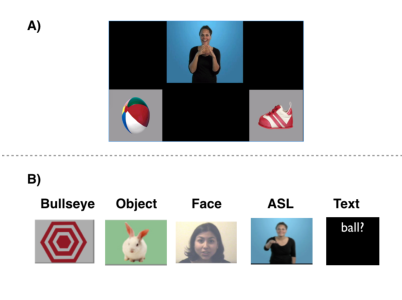
\includegraphics{figs/e1_stim-1} 

}

\caption[Stimuli for E1 and E2]{Stimuli for E1 and E2. Panel A shows the layout of the fixation locations for all tasks: the center stimulus, the target, and the distracter. Panel B shows the five center stimulus items: a static geometric shape (Bullseye), a static image of a familiar object (Object), a person speaking (Face), a person signing (ASL), and printed text (Text).}\label{fig:e1_stim}
\end{figure}
\end{CodeChunk}

\subsection{Method}\label{method}

\subsubsection{Participants}\label{participants}

\begin{table}[b]
\centering
\begin{tabular}{lrrrr}
  \hline
Task & Mean\_Age & Min\_Age & Max\_Age & n \\ 
  \hline
ASL & 27.90 & 16.00 & 53.00 &  30 \\ 
  Face & 26.00 & 25.00 & 26.00 &  24 \\ 
  Object & 31.90 & 26.00 & 39.00 &  40 \\ 
  Bullseye & 26.10 & 26.00 & 27.00 &  16 \\ 
   \hline
\end{tabular}
\caption{Age distributions of children in Experiment 1. All ages are reported in months.} 
\end{table}

Table 1 contains details about the age distributions of children in all
of four samples.

\emph{Spoken English samples.} Participants were 80 native, monolingual
English-learning children divided across three samples. Participants had
no reported history of developmental or language delay.

\emph{ASL sample.} Participants were 30 native, monolingual ASL-learning
children (18 deaf, 12 hearing). All children, regardless of hearing
status, were exposed to ASL from birth through extensive interaction
with at least one caregiver fluent in ASL and were reported to
experience at least 80\% ASL in their daily lives. The ASL sample
included a wider age range compared to the spoken English samples
because this is a rare population.

\subsubsection{Stimuli}\label{stimuli}

\emph{ASL linguistic stimuli.} We recorded two sets of ASL stimuli,
using two valid ASL sentence structures for questions: 1)
Sentence-initial wh-phrase: ``HEY! WHERE {[}target noun{]}?'' and 2)
Sentence-final wh-phrase: ``HEY! {[}target noun{]} WHERE?'' Two female
native ASL users recorded several tokens of each sentence in a
child-directed register. Before each sentence, the signer produced a
common attention-getting gesture. Mean sign length was 1.25 sec, ranging
from 0.69 sec to 1.98 sec.

\emph{English linguistic stimuli.} All three tasks (Object, Bullseye,
and Face) featured the same female speaker who used natural
child-directed speech and said: ``Look! Where's the (target word)?'' The
target words were: ball, banana, book, cookie, juice, and shoe. For the
Face task, a female native English speaker was video-recorded as she
looked straight ahead and said, ``Look! Where's the (target word)?''
Mean word length was 0.79 sec, ranging from 0.6 sec to 0.94 sec.

\emph{ASL and English visual stimuli.} The image set consisted of
colorful digitized pictures of objects presented in fixed pairs with no
phonological overlap (ASL task: cat---bird, car---book, bear---doll,
ball---shoe; English tasks: book-shoe, juice-banana, cookie-ball). Side
of target picture was counterbalanced across trials.

\subsubsection{Design and procedure}\label{design-and-procedure}

Children sat on their caregiver's lap and viewed the task on a screen
while their gaze was recorded using a digital camcorder. On each trial,
children saw two images of familiar objects on the screen for two
seconds before the center stimulus appeared (see Fig 1). Then they
processed the target sentence -- which consisted of a carrier phrase, a
target noun, and a question -- followed by two seconds without language
to allow for a response. Participants saw 32 test trials with several
filler trials interspersed to maintain interest.

\emph{Coding.} Participants' gaze patterns were coded (33-ms resolution)
as being fixated on either the center stimulus, one of the images,
shifting between pictures, or away. To assess inter-coder reliability,
25\% of the videos were re-coded. Agreement was scored at the level of
individual frames of video and averaged 98\% on these reliability
assessments.

\subsection{Results and Discussion}\label{results-and-discussion}

\subsubsection{Analysis plan}\label{analysis-plan}

First, we present behavioral analyses of First shift accuracy and
Reaction Time (RT). RT corresponds to the latency to shift away from the
central stimulus to either picture measured from target-noun onset.
Accuracy was the mean proportion of first gaze shifts that landed on the
target picture out of the total number of shifts. We log transformed all
RTs and used the \texttt{lme4} R package (Bates, Maechler, Bolker, \&
Walker, 2013) to fit mixed-effects regression models that included a
random intercept for each participant and item. Since children's age
varied across conditions, we included age in months as a covariate in
all models. All analysis code can be found in the online repository for
this project: \url{https://github.com/kemacdonald/speed-acc}.

Next, we present two exploratory model-based analyses to quantify
differences in eye movements across the four samples. First, we use an
EWMA method to model changes in accuracy as a function of increases in
RT. For each RT, the model generates two values: a ``control statistic''
(CS, which captures the running average accuracy of first shifts) and an
``upper control limit'' (UCL, which captures the pre-defined limit of
when accuracy would be categorized as above chance level). Here, the CS
is an expectation of random shifting to either the target or the
distracter image (nonlanguage-driven shifts), or a Bernoulli process
with probability of success 0.5. As the RTs get longer, we assume that
participants have gathered more information and should become more
accurate, or a Bernoulli process with probability success \textgreater{}
0.5. Using this model, we can quantify and compare: a) the cutoff point
when the CS exceeds the UCL, indicating that participants started to
generate language-driven shifts and b) the proportion of shifts that the
model categorizes as language-driven vs.~nonlanguage-driven.

Finally, we took the shifts that were categorized as language-driven by
the EWMA and fit a hierarchical Bayesian drift-diffusion model (HDDM) to
quantify differences in the speed and accuracy of language-driven eye
movements. We chose to implement a hierarchical Bayesian version of the
DDM using the HDDM Python package (Wiecki, Sofer, \& Frank, 2013) since
we had relatively few trials from child participants and recent
simulation studies have shown that the HDDM approach was better than
other DDM fitting methods for small data sets (Ratcliff \& Childers,
2015). The model assumes that people accumulate noisy evidence in favor
of one alternative with a response generated when the evidence crosses a
pre-defined decision threshold. Here we focus on two parameters of
interest that map onto meaningful psychological variables:
\emph{boundary separation}, which indexes the amount of evidence
gathered before a response (higher values suggest more cautious
responding) and \emph{drift rate}, which indexes the amount of evidence
accumulated per unit time (higher values suggest more efficient
processing).

\begin{CodeChunk}
\begin{figure}[t]

{\centering 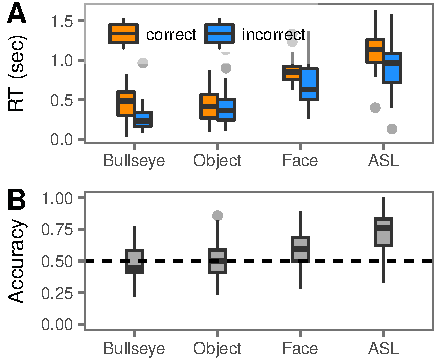
\includegraphics{figs/e1_acc_rt_plot-1} 

}

\caption[First shift accuracy and RTs from E1]{First shift accuracy and RTs from E1. Panel A shows a boxplot representing the distribution of RTs for correct (orange) and incorrect (blue) shifts for each center stimulus type. Panel B shows the distribution of mean first shift accuracy scores for each center stimulus type. The solid lines represent median values, the boundaries of the box show the upper and lower quartiles, and the whiskers show the full range of the data excluding outliers.}\label{fig:e1_acc_rt_plot}
\end{figure}
\end{CodeChunk}

\subsubsection{Behavioral analyses}\label{behavioral-analyses}

\emph{RT.} Visual inspection of the Fig 2, panel A suggests that there
was a speed accuracy tradeoff in the ASL, Face, and Bullseye conditions,
with incorrect shifts tending to be faster than correct shifts. To
quantify differences across the groups, we fit a linear mixed-effects
regression predicting first shift RT as a function of center stimulus
type, controlling for age, and including user-defined contrasts to test
specific comparisons of interest:
\texttt{Log(RT) $\sim$ center stimulus type + age +  (1 | subject) + (1 | item)}.
We found that (a) ASL learners generated slower RTs compared to all of
the spoken English samples (\(\beta\) = -0.97, \(p\) \textless{} .001),
(b) ASL learners' shifts were slower compared directly to participants
in the Face task (\(\beta\) = -0.42, \(p\) \textless{} .001), and (c)
participants in the Face task shifted slower compared to participants in
the Object and Bullseye tasks (\(\beta\) = -0.73, \(p\) \textless{}
.001).

\emph{Accuracy.} Next we compared the accuracy of first shifts across
the different tasks by fitting a mixed-effects logistic regression with
the same specifications and contrasts as the RT model. We found that (a)
ASL learners were more accurate compared to all of the spoken English
samples (\(\beta\) = -0.78, \(p\) \textless{} .001), (b) ASL learners
were more accurate when directly compared to participants in the Face
task (\(\beta\) = -0.62, \(p\) = 0.001), and (c) participants in the
Face task were numerically more accurate compared to participants in the
Object and Bullseye tasks (\(\beta\) = -0.73) but this effect was not
significant (\(p\) = 0.089).

\subsubsection{Model-based analyses}\label{model-based-analyses}

\emph{EWMA.} Figure 3 shows changes in the control statistic (CS) and
the upper control limit (UCL) as a function of participants' RTs. Each
CS starts at chance performance and below the UCL. In the ASL and Face
tasks, the CS value begins to increase with RTs around 0.7 seconds after
noun onset and eventually crosses the UCL, indicating that responses
\textgreater{} 0.7 sec were on average above chance levels. In contrast,
the CS in the Object and Bullseye tasks never crossed the UCL,
indicating that children's shifts were equally likely to land on the
target or the distracter, regardless of when they were initiated. This
result suggests that first shifts in the Bullseye/Object tasks were not
language-driven and may instead have reflected a different process such
as gathering more information about the referents in the visual world.

Next, we compared the EWMA output for participants in the ASL and Face
tasks. We found that ASL learners generated fewer shifts when the CS was
below the UCL (\(\beta\) = -1.61, \(p\) \textless{} .001), indicating
that a larger proportion of their initial shifts away were
language-driven (see the differences in the red shaded area in Fig 3).
We did not find evidence for a difference in the timing of when the CS
crossed the UCL (\(\beta\) = -0.04, \(p\) = 0.387), indicating that both
groups began to generate language-driven shifts about the same time
after noun onset.

\emph{HDDM.} Using the output of the EWMA, we compared the timing and
accuracy of language-driven shifts for participants in the ASL and Face
tasks.\footnote{We report the mean and the 95\% highest density interval
  (HDI) of the posterior distributions for each parameter. The HDI
  represents the range of credible values given the model specification
  and the data. We chose not to interpret the DDM fits for the
  Bullseye/Face tasks since there was no suggestion of any non-guessing
  signal.} We found that ASL learners had a higher estimate for the
boundary separation parameter compared to the Face participants (ASL
boundary = 1.77, HDI = {[}1.64, 1.9{]}; Face boundary = 1.35, HDI =
{[}1.21, 1.49{]}), with no overlap in the credible values (see Fig 4).
This suggests that ASL learners accumulated more evidence about the
linguistic signal before generating an eye movement. We found high
overlap for estimates of the drift rate parameter, indicating that both
groups processed the linguistic information with similar efficiency (ASL
drift = 0.64, HDI = {[}0.44, 0.83{]}; Face drift = 0.57, HDI = {[}0.33,
0.83{]}).

Taken together, the behavioral analyses and the EWMA/HDDM results
provide converging support that ASL learners were sensitive to the value
of eye movements, producing fewer nonlanguage-driven shifts and
prioritizing accuracy over speed, but accumulating information at
roughly the same rate. This behavior seems reasonable since the
potential for missing subsequent linguistic information is high if ASL
users shifted prior to gathering sufficient information. It is important
to point out that these were exploratory findings and that there were
several, potentially important differences between the stimuli,
apparatus, and populations. In E2, we set out to perform a
well-controlled, confirmatory test of our adaptive tradeoffs account.

\begin{CodeChunk}
\begin{figure}[t]

{\centering 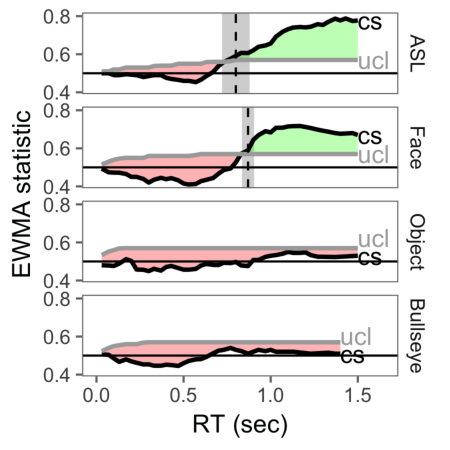
\includegraphics{figs/e1_control_chart-1} 

}

\caption[Output for the EWMA guessing model in E1]{Output for the EWMA guessing model in E1. The black curve represents the evolution of the control statistic (CS) as a function of reaction time. The grey curve represents the upper control limit (UCL). The vertical dashed line is the median cutoff value (point when the control process shifts out of a guessing state). The grey shaded area represents the 95\% confidence interval around the estimate of the median cutoff point. And the shaded areas represents the proprotion of responses that were flagged as guesses (red) and language-driven (green).}\label{fig:e1_control_chart}
\end{figure}
\end{CodeChunk}

\begin{CodeChunk}
\begin{figure}[t]

{\centering 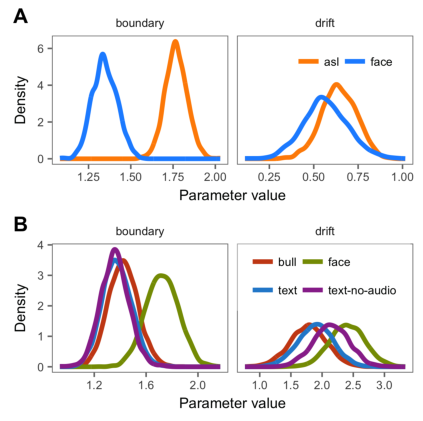
\includegraphics{figs/hddm_plot-1} 

}

\caption[Posterior distributions for the boundary and drift rate parameters for children in E1 (Panel A) and adults in E2 (Panel B)]{Posterior distributions for the boundary and drift rate parameters for children in E1 (Panel A) and adults in E2 (Panel B).}\label{fig:hddm_plot}
\end{figure}
\end{CodeChunk}

\section{Experiment 2}\label{experiment-2}

\begin{CodeChunk}
\begin{figure}[t]

{\centering 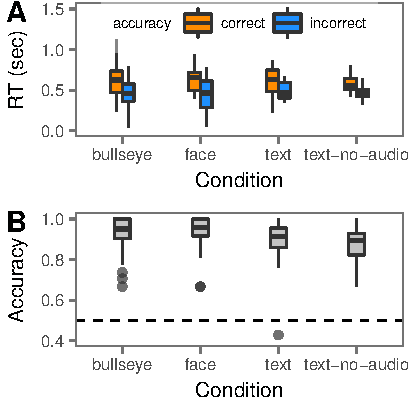
\includegraphics{figs/e2_plot_print-1} 

}

\caption[Behavioral results from E2]{Behavioral results from E2. All plotting conventions are the same as in Figure 2.}\label{fig:e2_plot_print}
\end{figure}
\end{CodeChunk}

\begin{CodeChunk}
\begin{figure}[t]

{\centering 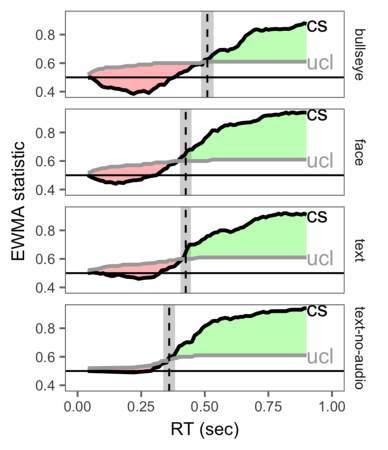
\includegraphics{figs/e2_control_chart-1} 

}

\caption[EWMA model output for E2]{EWMA model output for E2. All plotting conventions are the same as Figure 3.}\label{fig:e2_control_chart}
\end{figure}
\end{CodeChunk}

In E2, we attempt to replicate a key finding from E1: that increasing
the competition between fixating the language source and the
nonlinguistic visual world reduces nonlanguage-driven eye movements.
Moreover, we conducted a confirmatory test of our hypothesis that also
controlled for the population differences present in E1. We tested a
sample of English-speaking adults using a within-participants
manipulation of the center stimulus type. We used the Face and Bullseye
stimulus sets from E1 and added two new conditions: Text, where the
verbal language information was accompanied by a word-by-word display of
printed text (see Fig 1), and Text-no-audio, where the spoken language
stimulus was removed. We chose text processing since, like sign language
comprehension, the linguistic information is gathered via fixations to
the visual world.

Our key behavioral prediction is that participants in the Text
conditions should produce a higher proportion of language-driven shifts
as indexed by the EWMA model output. We did not have strong predictions
for the DDM parameter fits since the goal of the Text manipulation was
to modulate participants' strategic allocation of visual attention and
not the accuracy/efficiency of information processing.

\subsection{Method}\label{method-1}

\subsubsection{Participants}\label{participants-1}

25 Stanford undergraduates participated (5 male, 20 females) for course
credit. All participants were monolingual, native English speakers and
had normal vision.

\subsubsection{Stimuli}\label{stimuli-1}

Audio and visual stimuli were identical to the Face and Bullseye tasks
in E1. We included a new center fixation stimulus type: printed text.
The text was displayed in a white font on a black background and was
programmed such that only a single word appeared on the screen, with
each word appearing for the same duration as the corresponding word in
the spoken language stimuli.

\subsubsection{Design and procedure}\label{design-and-procedure-1}

The design was nearly identical to E1, with the exception of a change to
a within-subjects manipulation where each participant completed all four
tasks (Bullseye, Face, Text, and Text-no-audio). In the Text condition,
spoken language accompanied the printed text. In the Text-no-audio
condition, the spoken language stimulus was removed. Participants saw a
total of 128 trials while their eye movements were tracked using
automated eye-tracking software.

\subsection{Results and Discussion}\label{results-and-discussion-1}

\subsubsection{Behavioral analyses}\label{behavioral-analyses-1}

\emph{RT.} Visual inspection of Figure 5, panel A suggests that there
was a speed-accuracy tradeoff for all conditions: incorrect gaze shifts
tended to be faster than correct shifts. We fit a linear mixed-effects
regression with the same specification as in E1, but we added by-subject
intercepts and slopes for each center stimulus type to account for our
within-subjects manipulation. We did not find evidence that RTs were
different across conditions (all \(p\) \textgreater{} .05).

\emph{Accuracy.} Next, we modeled accuracy using a mixed-effects
logistic regression with the same specifications (see Panel B of Fig 5).
We found that adults' first shifts were highly accurate, and, in
contrast to the children in E1, their responses were above chance level
even in the Bullseye condition when the center stimulus was not salient
or informative. We also found that participants tended to be less
accurate in the Text conditions compared to conditions without text
(\(\beta\) = 1.18, \(p\) = 0.002). We did find not any other
statistically significant differences.

\subsubsection{Model-based analyses}\label{model-based-analyses-1}

\emph{EWMA.} For all four conditions, the CS crossed the UCL (see Fig
6), suggesting that for all tasks some proportion of adults' shifts were
language-driven. Interestingly, we found a graded effect of condition
(see the shift in the vertical dashed lines in Fig 5) on the point when
the CS crossed the UCL such that the Text-no-audio condition occurred
earliest (\(M_{text-no-audio}\) = 0.39), followed by the Text and Face
conditions that were not different from one another (\(M_{text}\) =
0.44, \(M_{face}\) = 0.45, \(p\) \textgreater{} .05), and finally the
Bullseye condition (\(M_{bullseye}\) = 0.54). We also found the same
graded difference in the proportion of shifts that occurred while the CS
was below the UCL (see the red vs.~green shaded area in Fig 5),
indicating a higher proportion of first shifts were language-driven in
the Text conditions, with the highest proportion in the Text-no-audio
condition when tested against the three other conditions
(\(M_{text-no-audio}\) = 3.88, \(\beta\) = 1.74, \(p\) \textless{}
.001). These results provide strong evidence for our key prediction:
that increasing the value of fixating the language source reduces
exploratory gaze shifts to the nonlinguistic visual world.

\emph{HDDM.} Using the output of the EWMA, we fit the same HDDM as in
E1. There was high overlap of the posterior distributions for the drift
rate parameters (see Fig 4, panel B), suggesting that participants
gathered the linguistic information with similar efficiency. We also
found high overlap in the distribution of credible boundary separation
estimates for the Bullseye, Text, and Text-no-audio conditions.
Interestingly, we found some evidence for a higher boundary separation
in the Face condition compared to the other three center stimulus types
(Face boundary = 1.72, HDI = {[}1.47, 1.97{]}; Bullseye boundary = 1.42,
HDI = {[}1.21, 1.65{]}; Text boundary = 1.38, HDI = {[}1.16, 1.6{]};
Text-no-audio boundary = 1.36, HDI = {[}1.15, 1.58{]}), suggesting that
adults higher accuracy in this condition was driven by accumulating more
information before generating a response.

Together, these results suggest that adults were sensitive to the
tradeoff between gathering different kinds of information. When
processing text, people generated fewer nonlanguage-driven shifts (EWMA
results) but their processing efficiency of the linguistic signal itself
did not change (HDDM results). Interestingly, we found a graded
difference in the EWMA results between the Text and Text-no-audio
conditions, with the lowest proportion of early, nonlanguage-driven
shifts occurring while processing text without the verbal stimuli. This
behavior makes sense; if the adults could rely on the auditory channel
to gather the linguistic information, then the value of fixating the
text display decreases. In contrast to the children in E1, adults were
highly accurate in the Bullseye condition, perhaps because they
construed the Bullseye as a center fixation that they \emph{should}
fixate, or perhaps they had better encoded the location/identity of the
two referents prior to the start of the target sentence.

\section{General Discussion}\label{general-discussion}

Language comprehension can be facilitated by fixating on relevant
features of the nonlinguistic visual world or on the speaker. But how do
we decide where to look? We propose that eye movements during language
processing reflect a sensitivity to the tradeoffs of gathering different
kinds of information. We found that young ASL-learners generated slower
but more accurate shifts away from a language source and produced a
smaller proportion of nonlanguage-driven shifts compared to spoken
language learners. We found the same pattern of behavior within a sample
of English-speaking adults processing displays of printed text compared
to spoken language. These results suggest that as the value of fixating
on a location to gather information about the linguistic signal
increases, eye movements to the \emph{rest} of the visual world become
less useful and occur less often.

Our work here attempts to synthesize results from different populations
and stimuli in a single framework, but it has several limitations that
we hope will pave the way for future work. First, we have not performed
a confirmatory test of the DDM findings: both ASL-learners (E1) and
adults processing language from a person (E2) prioritize accuracy over
speed. So these findings, while interesting, are preliminary. Second, we
do not know what might be driving the population differences in E1. It
could be that ASL-learners' massive experience dealing with competition
for visual attention leads to changes in the deployment of eye movements
during language comprehension. Or, it could be that the in-the-moment
constraints of processing a visual language cause different fixation
behaviors. Finally, we used a very simple visual world, with only three
places to look, and very simple linguistic stimuli, especially for the
adults in E2. Thus it remains an open question how these results might
scale up to more complex language information and visual environments.

This work attempts to integrate top-down, goal-based models of vision
(Hayhoe \& Ballard, 2005) with work on language-driven eye movements
(Allopenna et al., 1998). While we chose to start with two case studies
-- ASL and text processing -- we think the account is more general and
that there are many real world situations where people must negotiate
the tradeoff between gathering more information about language or about
the world: e.g., processing spoken language in noisy environments or at
a distance; or early in language learning when children are acquiring
new words and often rely on nonlinguistic cues to reference such as
pointing or eye gaze. Overall, we hope this work contributes to a
broader account of eye movements during language comprehension that can
explain fixation behaviors across a wider variety of populations,
processing contexts, and during different stages of language learning.

\section{Acknowledgements}\label{acknowledgements}

We are grateful to the families who participated in this research.
Thanks to Melina Wailing for help with data collection. This work was
supported by an NSF GRFP to KM and an NIDCD grant to AF and DC
(DC012505).

\section{References}\label{references}

\setlength{\parindent}{-0.1in} \setlength{\leftskip}{0.125in} \noindent

\hypertarget{refs}{}
\hypertarget{ref-allopenna1998tracking}{}
Allopenna, P. D., Magnuson, J. S., \& Tanenhaus, M. K. (1998). Tracking
the time course of spoken word recognition using eye movements: Evidence
for continuous mapping models. \emph{Journal of Memory and Language},
\emph{38}(4), 419--439.

\hypertarget{ref-altmann2007real}{}
Altmann, G., \& Kamide, Y. (2007). The real-time mediation of visual
attention by language and world knowledge: Linking anticipatory (and
other) eye movements to linguistic processing. \emph{Journal of Memory
and Language}, \emph{57}(4), 502--518.

\hypertarget{ref-bates2013lme4}{}
Bates, D., Maechler, M., Bolker, B., \& Walker, S. (2013). Lme4: Linear
mixed-effects models using eigen and s4. r package version 1.0-5.

\hypertarget{ref-hayhoe2005eye}{}
Hayhoe, M., \& Ballard, D. (2005). Eye movements in natural behavior.
\emph{Trends in Cognitive Sciences}, \emph{9}(4), 188--194.

\hypertarget{ref-macdonald2017realtime}{}
MacDonald, K., LaMarr, T., Corina, D. and, Marchman, V., \& Fernald, A.
(under review). Real-time lexical comprehension in young children
learning american sign language.

\hypertarget{ref-ratcliff2015individual}{}
Ratcliff, R., \& Childers, R. (2015). Individual differences and fitting
methods for the two-choice diffusion model of decision making.
\emph{Decision}, \emph{2}(4), 237--279.

\hypertarget{ref-tanenhaus1995integration}{}
Tanenhaus, M. K., Spivey-Knowlton, M. J., Eberhard, K. M., \& Sedivy, J.
C. (1995). Integration of visual and linguistic information in spoken
language comprehension. \emph{Science}, \emph{268}(5217), 1632.

\hypertarget{ref-vandekerckhove2007fitting}{}
Vandekerckhove, J., \& Tuerlinckx, F. (2007). Fitting the ratcliff
diffusion model to experimental data. \emph{Psychonomic Bulletin \&
Review}, \emph{14}(6), 1011--1026.

\hypertarget{ref-wiecki2013hddm}{}
Wiecki, T. V., Sofer, I., \& Frank, M. J. (2013). HDDM: Hierarchical
bayesian estimation of the drift-diffusion model in python.
\emph{Frontiers in Neuroinformatics}, \emph{7}, 14.

\end{document}
